
\documentclass[tikz]{standalone}

\begin{document}
\tikzset{man/.pic={
    \node[circle,fill,minimum size=5mm] (head) {};
    \node[rounded corners=2pt,minimum height=.8cm,minimum width=0.4cm,fill,below = 1pt of head] (body) {};
    \draw[line width=1mm,round cap-round cap] ([shift={(2pt,-1pt)}]body.north east) --++(-90:6mm);
    \draw[line width=1mm,round cap-round cap] ([shift={(-2pt,-1pt)}]body.north west)--++(-90:6mm);
    }}
\begin{tikzpicture}
    \pic[cyan] at (.5, -.5) (myman) {man};
    \node (p) at (.5, -2.5) {\textcolor{cyan}{\tiny{$p=(p_1, p_2, p_3, \dots, p_{15}, p_{16})$}}};
    \node at (.5, -3.5) (title) {\textcolor{cyan}{\tiny{memory-two}}};
    \node[align=center] (0) at (3, 0) {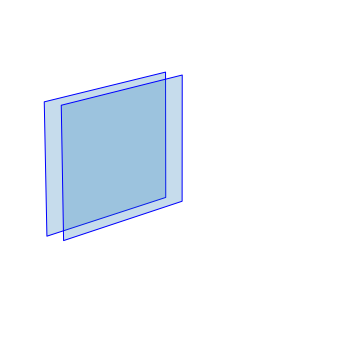
\includegraphics[width=.3\textwidth]{static/memory_two.png}};

    \coordinate  (A) at (.5, 0);
    \coordinate  (B) at (1.5, .5) ;
    \draw [->] (A.north) to [out=90,in=180] (B.north);

    \pause


    \pic[solarizedGreen] at (6.5, -.5) (myman) {man};
    \node (p) at (6.5, -2.5) {\textcolor{solarizedGreen}{\tiny{$p=(p_1, p_2, p_1, \dots, p_3, p_4)$}}};
    \node (p) at (6.5, -3.2) {\textcolor{solarizedGreen}{\tiny{$\tilde{p}=(p_1, p_2, p_3, p_4)$}}};
    \node at (6.5, -3.9) (title) {\textcolor{solarizedGreen}{\tiny{two-bit reactive}}};
    \node[align=center] (0) at (9, 0) {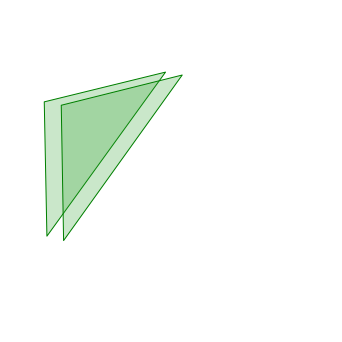
\includegraphics[width=.3\textwidth]{static/two_bits.png}};

    \coordinate  (A) at (6.5, 0);
    \coordinate  (B) at (7.5, .5) ;
    \draw [->] (A.north) to [out=90,in=180] (B.north);


    % \pic[solarizedGreen] at (12.5, -.5) (myman) {man};
    
    % \node[cloud,
    % draw =solarizedBase03,
    % text=solarizedBase03,
    % minimum width = 1mm,
    % minimum height = 1mm,
    % inner sep=1.1mm] (c) at (11.3, 0) {\tiny{$\frac{16}{4}$}};
    % \node (p) at (12.5, -2.5) {\textcolor{solarizedGreen}{\tiny{$p=(1, p_2, 1, \dots, p_3, p_4)$}}};
    % \node (p) at (12.5, -3.2) {\textcolor{solarizedGreen}{\tiny{$\tilde{p}=(1, p_2, p_3, p_4)$}}};
    % \node at (12.5, -3.9) (title) {\textcolor{solarizedGreen}{\tiny{\textbf{agreeable} two-bit reactive}}};
    % \node[align=center] (0) at (16, 0) {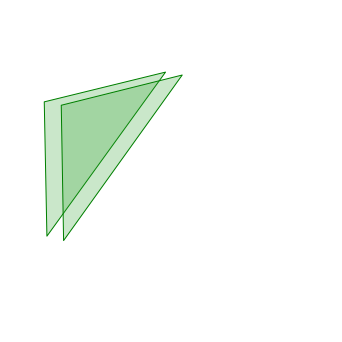
\includegraphics[width=.13\textwidth]{static/two_bits.png}};
    % \node[align=center] (0) at (12.5, -1.2) {
\includegraphics[width=.01\textwidth]{static/medal.png}};
    

    % \coordinate  (A) at (12.5, 0);
    % \coordinate  (B) at (13.5, .5) ;
    % \draw [->, solarizedOrange, thicko] (A.north) to [out=90,in=180] (B.north);
\end{tikzpicture}
\end{document}